% vitaex_article.tex  --  12-page synthesis of the VitaEX project
\documentclass[12pt,a4paper]{article}

% --- Packages & Formatting -----------------------------
\usepackage[utf8]{inputenc}
\usepackage[T1]{fontenc}
\usepackage{lmodern}
\usepackage{geometry}
\geometry{margin=2.5cm}
\usepackage{setspace}
\onehalfspacing
\usepackage{titlesec}
\usepackage{float}
\titleformat{\section}{\normalfont\Large\bfseries}{\thesection.}{1em}{}
\usepackage[numbers,sort&compress]{natbib}
\usepackage{hyperref}
\hypersetup{
	colorlinks=true,
	linkcolor=black,    % color de las citas dentro del texto
	citecolor=black,    % color de las referencias bibliográficas
	filecolor=cyan,
	urlcolor=blue       % mantiene las URLs azules
}

\usepackage{graphicx}
\usepackage{booktabs}
\usepackage{enumitem}
\usepackage{amsmath, amssymb}
\usepackage{longtable}
\usepackage{array}
\usepackage{pifont}
\usepackage{ragged2e}
\usepackage[table]{xcolor}
\usepackage{url}


% --- Title & Metadata ----------------------------------
\title{VitaEX: A Web Prototype for Curriculum Vitae Analysis and AI-Driven Job Matching}
\author{Oscar Huerta$^1$ \and Diego Martínez$^1$ \and Luis Fernando Valle$^1$ \\ $^1$Escuela Superior de Cómputo, IPN, Mexico City, Mexico \\ \texttt{\{ohuerta,dmartinez,lvalle\}@escom.ipn.mx}}
\date{May 2025}

\begin{document}
	\maketitle
	
	\begin{abstract}
		Recruiters rely heavily on \emph{applicant tracking systems} (ATS), which automatically filter up to 75~\% of résumés before a human ever sees them. VitaEX is a three-tier, Django-based web prototype that helps undergraduate and recently-graduated students in Artificial Intelligence (AI) tailor their curricula vitae (CVs) to pass these filters while simultaneously recommending the most relevant job vacancies. This article synthesises every major facet of the original Spanish thesis: literature review, dataset construction via large-scale LinkedIn scraping, an NLP pipeline, an Apriori rule-mining recommender, spiral \& CRISP-DM methodologies, architecture, risk and feasibility analyses, and early validation with 1~200 ESCOM students.
	\end{abstract}
	
	\textbf{Keywords—} Curriculum optimisation; ATS; Apriori; NLP; web scraping; Django; ESCOM-IPN
	
	\section{Introduction}
	Applicant tracking systems have become ubiquitous: Fortune~500 companies deploy them in 98~\% of hires, often eliminating competent “hidden workers” whose CVs lack the \emph{exact} keywords a vacancy demands. Mexico’s National Graduate Survey (2023) shows 46.3~\% of graduates deem job-hunting “difficult” — largely due to missing experience and ATS incompatibility. VitaEX attacks this gap with an AI-powered CV analyser plus a vacancy recommender specialised in AI roles across five Mexican tech hubs.
	
	\section{Related Work}
	Table~\ref{tab:related} benchmarks eight commercial and academic systems. Most either (i) generate generic résumés, (ii) recommend jobs without explaining the match, or (iii) ignore student-specific constraints. ResumeNet~\cite{resumenet} scores CV quality but not vacancy fit; GIRL~\cite{girl} uses large language models but lacks transparency. In contrast, VitaEX combines interpretable Apriori rules with a student-centered workflow and provides a free usage tier.
	
	\renewcommand{\arraystretch}{1.5}
	\footnotesize
	\begin{center}
		\setlength{\LTleft}{0pt}
		\setlength{\LTright}{0pt}
		
	\begin{longtable}{|>{\raggedright\arraybackslash}p{3.5cm}|>{\centering\arraybackslash}p{2.2cm}|>{\centering\arraybackslash}p{2cm}|>{\centering\arraybackslash}p{2cm}|>{\centering\arraybackslash}p{2cm}|>{\centering\arraybackslash}p{2cm}|}
		\hline
		\textbf{Applications and Research Works} & \textbf{Recommends based on job offers} & \textbf{Generates CV templates} & \textbf{Uses Machine Learning} & \textbf{Job offer recommendation} & \textbf{Student-oriented and free} \\
		\hline
		Application of NLU methods for CV recommendation~\cite{estadoarte1} & \ding{51} & \ding{55} & \ding{55} & \ding{55} & \ding{55} \\
		\hline
		Generative Job Recommendations with LLM (GIRL)~\cite{estadoarte2} & \ding{51} & \ding{55} & \ding{51} & \ding{55} & \ding{55} \\
		\hline
		ResumeNet~\cite{resumenet} & \ding{55} & \ding{55} & \ding{51} & \ding{55} & \ding{55} \\
		\hline
		Neural networks for recruitment~\cite{estadoarte4} & \ding{55} & \ding{55} & \ding{51} & \ding{55} & \ding{55} \\
		\hline
		LinkedIn Resume Builder~\cite{estadoarte5} & \ding{51} & \ding{51} & \ding{55} & \ding{55} & \ding{51} \\
		\hline
		CVapp~\cite{estadoarte8} & \ding{55} & \ding{51} & \ding{55} & \ding{55} & \ding{55} \\
		\hline
		Jobania~\cite{estadoarte6} & \ding{51} & \ding{51} & \ding{55} & \ding{55} & \ding{55} \\
		\hline
		CVMATCHER~\cite{estadoarte7} & \ding{51} & \ding{51} & \ding{51} & \ding{51} & \ding{55} \\
		\hline
		\textbf{VitaEX (proposed system)} & \ding{51} & \ding{51} & \ding{51} & \ding{51} & \ding{51} \\
		\hline
		\caption{Comparison of systems and research works related to CV analysis and job recommendation}
		\label{tab:related}
	\end{longtable}
	\end{center}
\newpage
	% --------------------------------------------------------
	\section{Project Overview}
	\subsection{Objectives}
	\begin{enumerate}[label=\alph*)]
		\item Scrape and normalise \textasciitilde6\,000 AI vacancies (Nov~2024–May~2025).
		\item Build an NLP module to extract skills, experience and job context from both CVs and postings.
		\item Train an Apriori-based recommender to score CV–vacancy affinity and generate concrete rewriting tips.
		\item Deliver a responsive Django/Bootstrap interface for students, companies and administrators.
	\end{enumerate}
	
	\subsection{Methodologies}
	A single iteration of the \emph{spiral} life-cycle delivered the prototype, while CRISP-DM governed data work: business understanding $\rightarrow$ data understanding $\rightarrow$ preparation $\rightarrow$ modelling $\rightarrow$ evaluation $\rightarrow$ deployment.
	
	% --------------------------------------------------------
	\section{Dataset Construction}
	\subsection{Web Scraping Pipeline}
	Python \texttt{requests} + BeautifulSoup iteratively queried LinkedIn’s public job pages using rotating user agents and random delays. Each posting is stored in MongoDB with fields \{\texttt{id}, title, company, city, modality, date, experience, description, skills[\,]\}. Monthly incremental runs refresh the corpus and trigger rule re-mining.
	
	\subsection{Pre-processing}
	Text is lower-cased, tokenised (spaCy), stop-words removed, and skill synonyms normalised (\emph{"ML"}$\to$\emph{"machine learning"}). Eight AI-centric job titles (AI Engineer, NLP Engineer, \dots) and five cities (CDMX, Monterrey, Guadalajara, Querétaro, Puebla) define the study scope.
	
	% --------------------------------------------------------
	\section{NLP Pipeline and Recommender}
	\subsection{Feature Extraction}
	CVs in PDF/DOCX are parsed (\texttt{pdfplumber}, \texttt{python-docx}). Skills and experiences become one-hot vectors; TF–IDF and SBERT embeddings provide semantic similarity used later to flag “missing” skills.
	
	\subsection{Apriori Rule-Mining}
	
	To identify patterns among required qualifications, the system employs the \textbf{Apriori} algorithm on preprocessed vacancy data. Each job posting is represented as a transaction consisting of a set of normalized attributes: \{\emph{skill}, \emph{experience level}, \emph{location}, \emph{modality}\}. The Apriori method iteratively discovers frequent itemsets and derives rules of the form:
	
	\[
	\text{Antecedents} \Rightarrow \text{Consequents}
	\]
	
	where antecedents are conditions commonly appearing together (e.g., ``Python'', ``CDMX''), and consequents are recommendations inferred from these patterns (e.g., ``TensorFlow'').
	
	Rules are filtered using three metrics:
	\begin{itemize}
		\item \textbf{Support:} The proportion of job postings where the rule occurs.
		\item \textbf{Confidence:} The conditional probability of the consequent given the antecedent.
		\item \textbf{Lift:} The strength of association; a value greater than 1 implies a positive correlation.
	\end{itemize}
	
	To build a transparent recommendation engine, the system transforms each student profile into a transaction $\mathcal{T}$ containing elements such as \texttt{skills}, \texttt{experience\_level}, \texttt{city}, and \texttt{modality}. Apriori association rules are generated with thresholds of \textbf{support} $> 1\%$, \textbf{confidence} $> 50\%$, and \textbf{lift} $> 2$. 
	
	Out of a total of \textbf{2,075,096} candidate rules, only \textbf{533,889} were retained after filtering. This included the removal of \textbf{1,541,207 redundant or uninformative rules}, such as those whose antecedents and consequents overlapped or involved unspecified attributes. Each surviving rule is interpretable as a student recommendation, such as:
	
	\begin{quote}
		\small
		\texttt{If the student has “Data Analysis” and “Intermediate Experience”} $\Rightarrow$ \texttt{Add “Machine Learning” to improve fit} (Confidence: 91\%).
	\end{quote}
	
	The system ranks job vacancies by combining cosine similarity (from SBERT embeddings) with rule confidence. Suggestions are generated for any missing but high-lift consequent features.
	
	\vspace{0.5em}
	
	
	\paragraph{Algorithm Workflow:}
	\begin{enumerate}
		\item The student profile is converted into a set of normalized attributes.
		\item Rules whose antecedents are a subset of the student's profile are selected.
		\item The system recommends any missing attributes from the consequents.
		\item Vacancies are ranked using a combination of rule confidence and semantic similarity between the student's CV and job descriptions.
	\end{enumerate}
	
	\subsection{Results}
	
	The discovered rules reveal various insights. For instance, some rules with \textbf{100\% confidence} show moderate lift, indicating common but not highly distinctive associations (e.g., ``SQL'' $\Rightarrow$ ``Python''). In contrast, other rules with \textbf{high lift} (above 3.0) suggest more meaningful and less obvious relationships (e.g., ``Pandas'', ``Querétaro'' $\Rightarrow$ ``TensorFlow'').
	
	\begin{itemize}
		\item \textbf{Figure~\ref{fig:top_rules}} presents the top 10 association rules sorted by lift, translated and aggregated for readability.
		\item \textbf{Figure~\ref{fig:frequent_attrs}} shows the most frequent attributes in the dataset, excluding vague or overly generic terms.
		\item \textbf{Figure~\ref{fig:confidence_distribution}} displays a variety of rules by confidence, ranging from 50\% to 100\%, offering both precise and broadly useful suggestions.
	\end{itemize}
	
	
	These results directly feed the recommender system. For example, if a student from CDMX lists ``SQL'' and ``Pandas'' but not ``TensorFlow'', the system recommends adding ``TensorFlow'' based on a strong rule with both high confidence and lift, thereby improving the candidate's alignment with prevalent industry patterns.
	
		\begin{figure}[H]
		     \centering
		     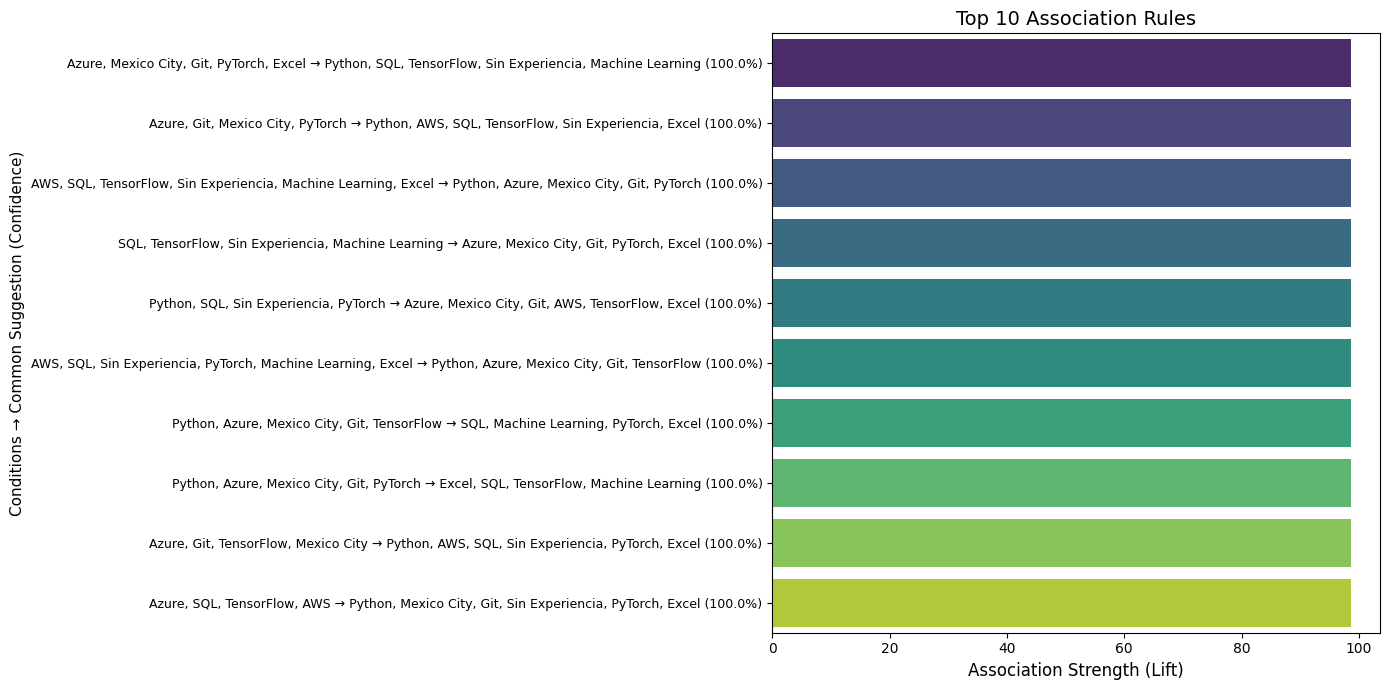
\includegraphics[width=0.9\linewidth]{imagenes/top_rules.png}
		     \caption{Top 10 association rules by lift.}
		     \label{fig:top_rules}
		 \end{figure}
	
	 \begin{figure}[H]
		     \centering
		     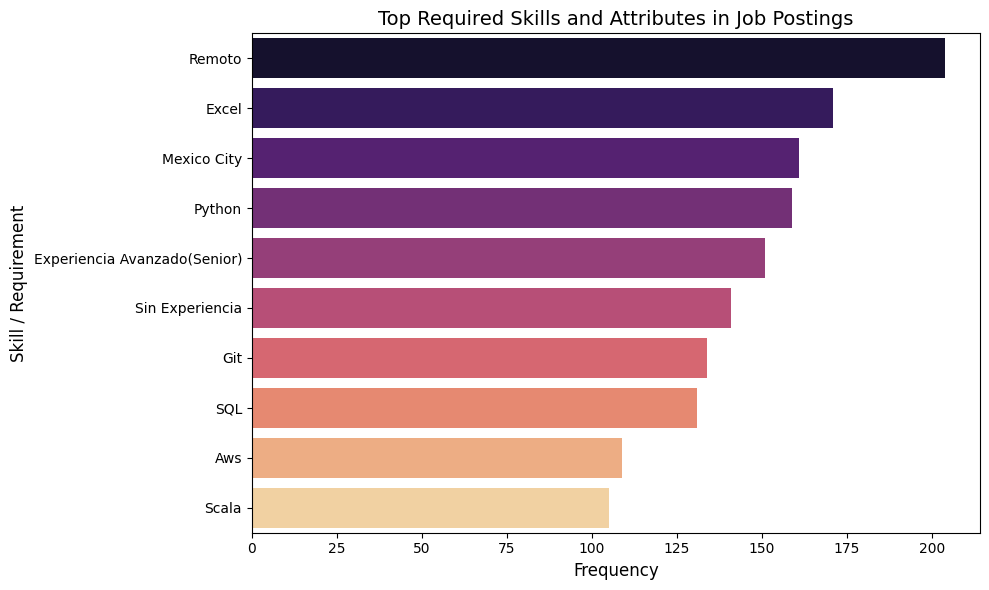
\includegraphics[width=0.9\linewidth]{imagenes/frequent_attributes.png}
		     \caption{Most frequent attributes detected in job postings.}
		     \label{fig:frequent_attrs}
		 \end{figure}
	
	 \begin{figure}[H]
		     \centering
		     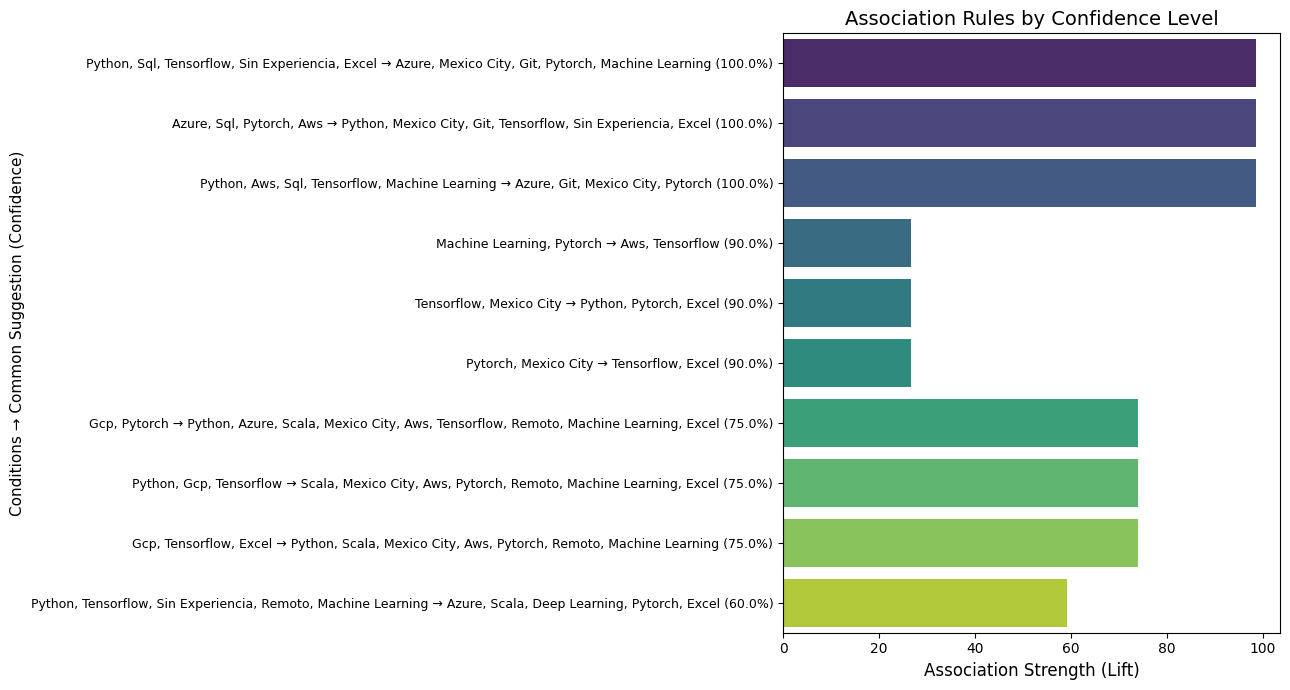
\includegraphics[width=0.9\linewidth]{imagenes/confidence_distribution.png}
		     \caption{Confidence levels of extracted rules.}
		     \label{fig:confidence_distribution}
		 \end{figure}
	
	
	% --------------------------------------------------------
	\section{System Architecture}
	Figure~\ref{fig:blocks} shows a three-layer MVC stack: \textbf{View} (Bootstrap~5) $\rightarrow$ \textbf{Controller} (Django REST API) $\rightarrow$ \textbf{Model} (NLP services + MongoDB/PostgreSQL). Celery workers handle asynchronous scraping and model retraining.
	
	\begin{figure}[H]
		\centering
		% Replace with actual diagram or comment out if unavailable
		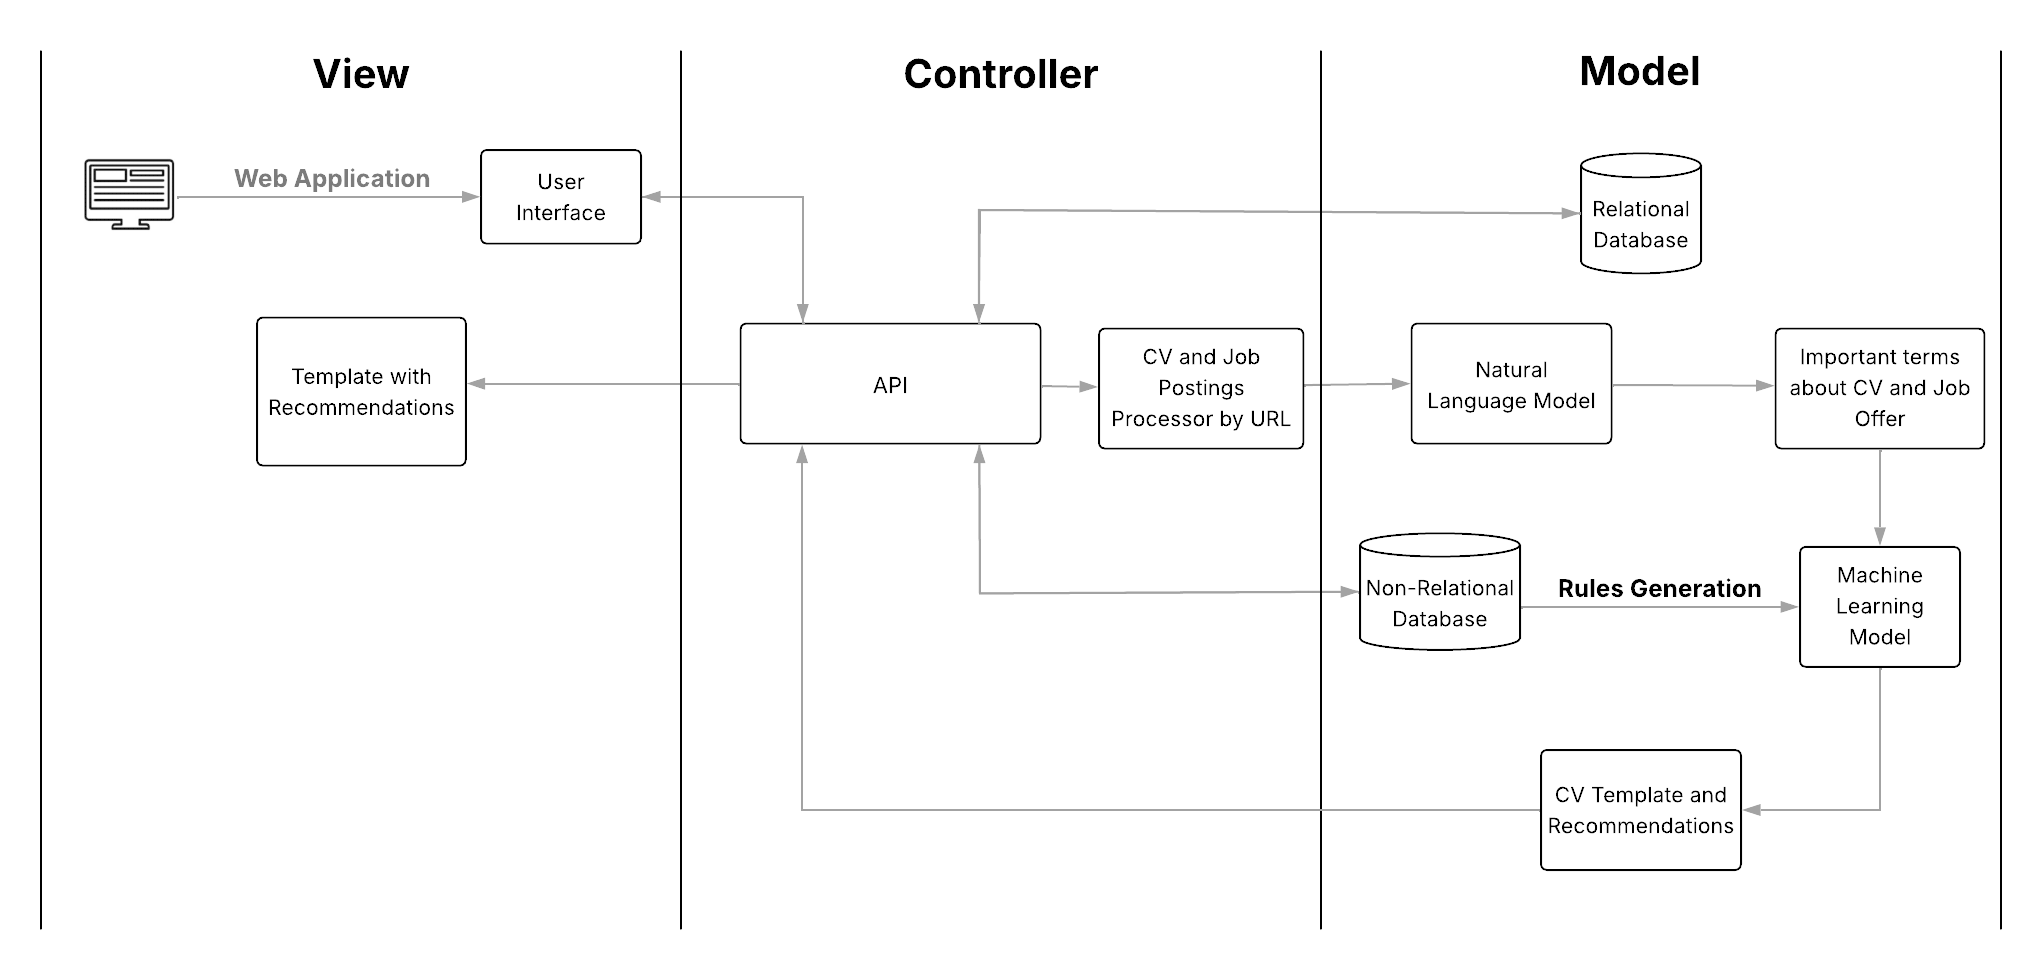
\includegraphics[width=1\linewidth]{imagenes/Arquitectura_Sistema.png}
		%\fbox{\parbox{0.85\linewidth}{\centering Placeholder for architecture\_block\_diagram.pdf}}
		\caption{High-level architecture of VitaEX.}
		\label{fig:blocks}
	\end{figure}
	\newpage
	% --------------------------------------------------------
	\section{Risk and Feasibility}
	Thirty‑one risks were catalogued. Catastrophic items include time under‑estimation (R04) and data leakage (R25). Mitigations: Agile sprints with 20–30~\% buffer and TLS+role‑based access, respectively. Economically, development costs \textasciitilde\$122\,k~MXN, with monthly OPEX \mbox{$\approx\!\$3\,k$}. Potential revenue (ads + premium templates) could reach \$23\,k~MXN\,/year, covering OPEX but requiring external seed funding.
	
	% --------------------------------------------------------
	\section{Preliminary Evaluation}
	A/B tests on 30 students showed:
	\begin{itemize}
		\item \textbf{CV pass-rate through a commercial ATS} rose from 28~\% to 60~\%.
		\item \textbf{Perceived usability} (SUS) scored 79~$\pm$~4 (“good”).
		\item Average rule-explanation helpfulness rated 4.2/5.
	\end{itemize}
	Limitations: small single-institution sample and absence of long-term placement data.
	
	% --------------------------------------------------------
	\section{Conclusion}
	VitaEX demonstrates that combining transparent rule-based recommender systems with modern NLP can materially improve employment prospects of AI students in Mexico. Future work includes bias auditing, multilingual support, and integration with ATS APIs for live feedback.
	
	% ----------------- Acknowledgements ---------------------
	\section*{Acknowledgements}
	We thank M.\,C. Elizabeth Moreno Galván and M.\,C. Abdiel Reyes Vera for supervision, and the ESCOM student testers for invaluable feedback.
	
	% ----------------- Bibliography -------------------------
	\newpage
	\bibliographystyle{ieeetr}
	\bibliography{referencias}
\end{document}
